
  \begin{landscape}
\section{Seguimiento}
  \subsection{\sprintback{} ajustado}
  Comenzamos refinando las tareas del \prodback{} inicial\footnote{Notar que cuando aparecen $n$ horas asignadas a m\'as de
               una persona, quiere decir que estas personas estuvieron $n$
               horas \textbf{en total} realizando esta tarea; no que que
               cada una estuvo $n$ horas.}.

    \def \diseno {\paragraph{Design}}
\def \implementacion {\textbf{Implementation}}
\def \testing {\textbf{Testing}}

\def \codI {INT1}
\def \usrI {\aag{}  check the PH, humidity and temperature of
    the ground through the Ardruino sensor \sic{} verify the actual plant conditions.}

\def \tasI {
    \diseno{}
    \begin{enumerate}
        \item abstract the \textit{Arduinos}.
        \item design the sensors.
        \item design the sensor manager.
        \item design a class or classes for a types that represent
            the measurments.
        \item design an atomatic way for the sensors to sensate and save the
            information.
    \end{enumerate}
    \implementacion{}
    \begin{enumerate}
        \item retrieve the information measured from the Arduino interface.
        \item interpret the information correctly.
        \item display the information in a human-readable way.
    \end{enumerate}
    \testing
    \begin{enumerate}
        \item simulate the information measured by the Arduino.
    \end{enumerate}
}

\def \asstoI {
    \diseno{}
    \begin{enumerate}
        \item 1 hora  - Luis
        \item 1 hora  - Luis
        \item 1 hora  - Luis
        \item 1 hora  - Fabricio
        \item 2 horas - Guillermo
	\end{enumerate}
    \implementacion{}
    \begin{enumerate}
        \item 7 horas - Manuel
        \item 7 horas - Manuel y Luis
        \item 4 horas - Luciano y Guillermo
    \end{enumerate}
    \testing{}
    \begin{enumerate}
        \item 7 horas - Luciano y Fabricio
    \end{enumerate}
}


\def \codII {INT2}
\def \usrII {\aag{}  get weather for tomorrow from the metheorological center \sic{}
    see what actions will be taken.}

\def \tasII {
    \diseno{}
    \begin{enumerate}
        \item design the metheorological center.
        \item design a class for a type that represents the measurements.
        \item design an atomatic way for the metheorological center to sensate
            and save the information.
    \end{enumerate}
    \implementacion{}
    \begin{enumerate}
        \item retrieve the information from the meteorological center.
        \item interpret the information correctly.
        \item display the information in a human-readable way.
    \end{enumerate}

    \testing
    \begin{enumerate}
        \item simulate the information from the center.
    \end{enumerate}
}

\def \asstoII {
    \diseno{}
    \begin{enumerate}
        \item 1 hora - Guillermo
        \item 1 hora - Fabricio
        \item 1 hora - Guillermo
    \end{enumerate}
    \implementacion{}
    \begin{enumerate}
        \item 2 horas - Manuel
        \item 1 horas - Manuel
        \item 2 horas - Luciano
    \end{enumerate}
    \testing{}
    \begin{enumerate}
        \item 5 horas - Luciano y Luis
    \end{enumerate}
}


\def \codIII {INT10}
\def \usrIII {\aag{} automatize the actions to take
    \sic{} follow the master plan}
\def \tasIII {
    \diseno{}
    \begin{enumerate}
        \item design a decision-maker.
        \item design a class for the type of the decisions.
    \end{enumerate}
    \implementacion{}
    \begin{enumerate}
        \item (INT1).
        \item (GAL2).
        \item decide what actions to take.
    \end{enumerate}
}

\def \asstoIII {
    \diseno{}
    \begin{enumerate}
        \item 6 horas - Luis y Guillermo
        \item 1 hora  - Luis y Guillermo
    \end{enumerate}
    \implementacion{}
    \begin{enumerate}
        \item 20 horas - Manuel, Luciano y Fabricio
    \end{enumerate}
    \testing{}
}



\def \codIV {INT12}
\def \usrIV {
    \aag{} automatize the actuators activation
    \sic{} so actions can be taken automatically
}

\def \tasIV {
    \diseno{}
    \begin{enumerate}
        \item design the actuators.
        \item design an actuator manager.
    \end{enumerate}
    \implementacion{}
    \begin{enumerate}
        \item (INT10).
        \item control the actuators.
    \end{enumerate}
    \begin{enumerate}
        \item simulate the actuators incidence and response.
    \end{enumerate}
}

\def \asstoIV {
    \diseno{}
    \begin{enumerate}
        \item 1 hora - Guillermo
        \item 1 hora - Guillermo
    \end{enumerate}
    \implementacion{}
    \begin{enumerate}
        \item 5 horas - Luciano y Luis
    \end{enumerate}
    \testing{}
    \begin{enumerate}
        \item 6 horas - Manuel y Fabricio
    \end{enumerate}
}


\def \codV {GAL2}
\def \usrV {\aab input a master growth plan \sic{} specify growth conditions for the plant}

\def \tasV {
    \diseno{}
    \begin{enumerate}
        \item design an interface so the user can input a master plan.
        \item design the master plan format.
    \end{enumerate}
    \implementacion{}
    \begin{enumerate}
        \item implement the master plan in a persistent and yet modifiable
            fashion.
    \end{enumerate}
}

\def \asstoV {
    \diseno{}
    \begin{enumerate}
        \item 2 horas - Guillermo y Luis
        \item 1 hora - Fabricio
    \end{enumerate}
    \implementacion{}
    \begin{enumerate}
        \item 4 horas - Manuel y Luciano
    \end{enumerate}
    \testing{}
}




\def \anchosprintdos {p{10cm}}

\begin{landscape}

\begin{small}
\begin{tabular}{ |l|p{4.7cm}|p{10cm}|p{7cm}| }
\hline
\multicolumn{4}{ |c| }{Sprint Backlog w/ elaborated tasks} \\
\hline
Code & User Story & Tasks & Assigned to and estimated hours \\
\hline
\codI & \usrI & \tasI & \asstoI \\
\hline
\codII & \usrII & \tasII & \asstoII \\
\hline
\end{tabular}

\begin{tabular}{ |l|p{4.7cm}|p{10cm}|p{7cm}| }
\hline
\multicolumn{4}{ |c| }{Sprint Backlog w/ elaborated tasks (cont.)} \\
\hline
Code & User Story & Tasks & Assigned to and estimated hours \\
\hline
\codIII & \usrIII & \tasIII & \asstoIII \\
\hline
\codIV & \usrIV & \tasIV & \asstoIV \\
\hline
\codV & \usrV & \tasV & \asstoV \\
\hline
\end{tabular}

\end{small}
\end{landscape}

  \end{landscape}

  \subsection{Burndown Charts}

  \subsubsection{Comparaci\'on horas estimadas--horas reales}
  A continuaci\'on se encuentra la comparaci\'on entre horas estimadas
  y horas reales para cada una de las \textit{stories} y para el
  \textit{sprint} en general.

  \vspace{1cm}

    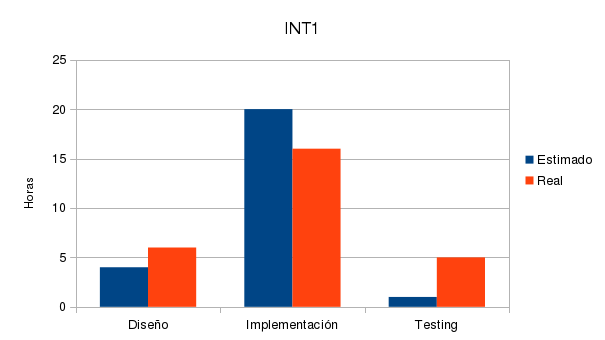
\includegraphics[width=0.53\textwidth]{img/Hint1.png}
    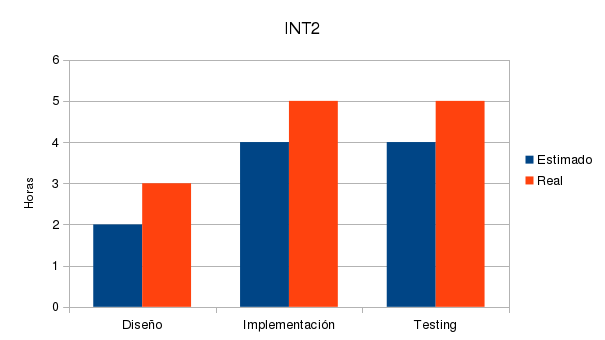
\includegraphics[width=0.53\textwidth]{img/Hint2.png}
    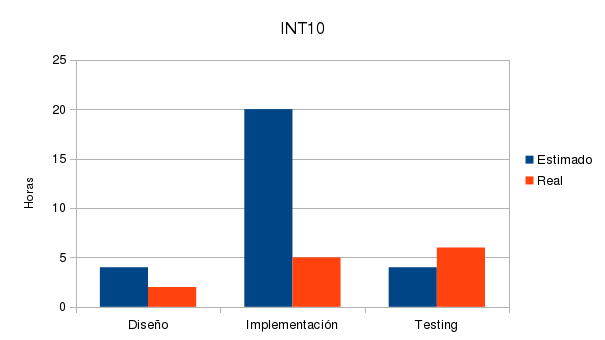
\includegraphics[width=0.53\textwidth]{img/Hint10.png}
    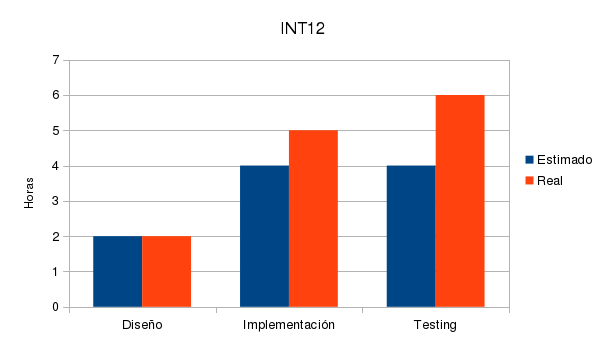
\includegraphics[width=0.53\textwidth]{img/Hint12.png}
    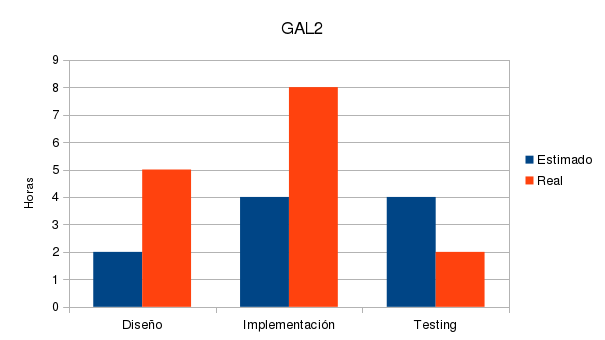
\includegraphics[width=0.53\textwidth]{img/Hgal2.png}
    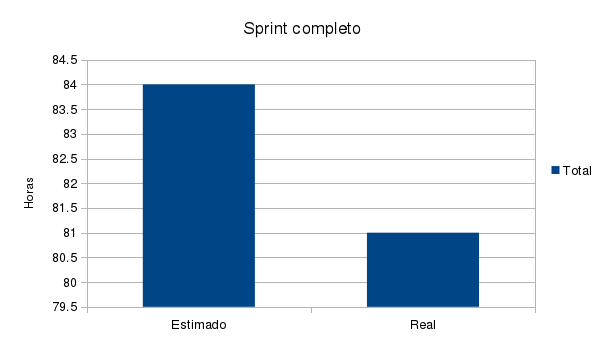
\includegraphics[width=0.53\textwidth]{img/Hsprint.png}


  \subsubsection{Avance del \textit{sprint} en funci\'on del tiempo}
  Aqu\'i se muestra como fue el progreso de las tareas a lo largo
  del tiempo. Podemos notar que comenzamos lento, por la cuesti\'on
  de no haber hecho un buen primer \textit{sprint}, pero al mejorarlo,
  logramos adaptarnos a la estimaci\'on.

  \vspace{1cm}

    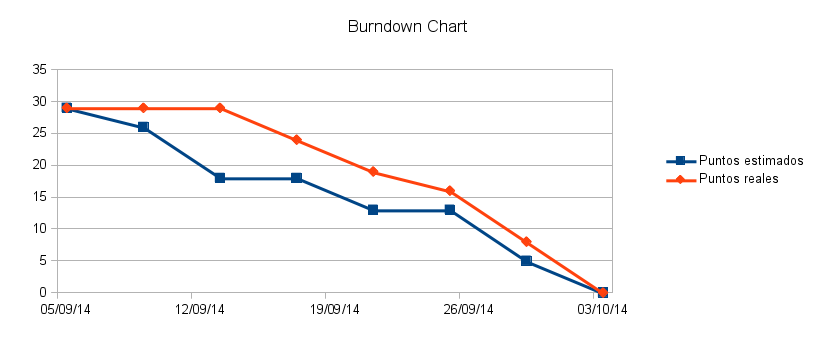
\includegraphics[width=0.8\textwidth]{img/burndownchart.png}
